\documentclass[14pt]{extarticle}
\usepackage{fontspec}
\usepackage{polyglossia}
\usepackage{amsmath}
\usepackage{amssymb}
\usepackage{xcolor}
\usepackage{fancyhdr}
\usepackage{graphicx}
\usepackage{listings}
\usepackage[most]{tcolorbox}
% \usepackage{setspace}
\usepackage{pifont}
\usepackage{enumitem}
\usepackage{titlesec}
\usepackage[bottom]{footmisc}
\usepackage{titling}
\usepackage{minted}
\usepackage{etoolbox}
\usepackage{array}
\usepackage{extsizes}
\usepackage{float}
\usepackage{booktabs}
\usepackage{hyperref}
\usepackage[onehalfspacing]{setspace}
\newif\ifcolorblind
\ifdefined\setcolorblind
  \setcolorblind
\fi

\ifcolorblind
  \usepackage[a4paper, landscape, top=1cm, bottom=1cm, left=1cm, right=1cm, headheight=1.5cm, headsep=0.5cm]{geometry}
\else
  \usepackage[a4paper, top=2.7cm, bottom=2.7cm, left=2.5cm, right=2.5cm, headheight=1.5cm, headsep=0.5cm]{geometry}
\fi
\usepackage{tikz}
\usepackage{datetime2}

\usetikzlibrary{automata, positioning, arrows.meta, arrows}

\newfontfamily\emoji{Segoe UI Emoji}

\pagestyle{fancy}

\setmainlanguage[numerals=western]{arabic}
\setotherlanguage{english}
\newfontfamily\arabicfont[Script=Arabic]{Calibri}
\newfontfamily\arabicfonttt[Script=Arabic]{Courier New}



\ifcolorblind
\lstset{
  language=[Sharp]C,
  numbers=left,
  stepnumber=1,
  numbersep=8pt,
  frame=single,
  basicstyle=\ttfamily\small,
  keywordstyle=\bfseries,
  stringstyle=\ttfamily,
  commentstyle=\itshape
}
\else
\lstset{
  language=[Sharp]C,
  numbers=left,
  stepnumber=1,
  numbersep=8pt,
  frame=single,
  basicstyle=\ttfamily\small,
  keywordstyle=\color{blue},
  stringstyle=\color{red},
  commentstyle=\color{green!50!black}
}
\fi

\newif\ifdetailed
\ifdefined\setdetailed
  \setdetailed
\fi

\newif\ifwithsols
\ifdefined\setwithsols
  \setwithsols
\fi

\ifcolorblind
  \AtBeginDocument{
    \LARGE
    \usemintedstyle{bw}
  }
\fi

% unified tcolorboxes for articles
\ifcolorblind
\tcbset{colback=white, colframe=black, fonttitle=\bfseries, boxrule=1pt}
\newtcolorbox{boxDef}[1][]{title={{\emoji📘} تعريف\ifx\\#1\\\else ~#1\fi :}}
\newtcolorbox{boxExercise}[1][]{title={{\emoji🧩} تمرين\ifx\\#1\\\else ~#1\fi :}}
\newtcolorbox{boxExample}[1][]{title={{\emoji📝} مثال\ifx\\#1\\\else ~#1\fi :}}
\newtcolorbox{boxNote}[1][]{title={{\emoji✨} ملاحظة\ifx\\#1\\\else ~#1\fi :}}
\newtcolorbox{boxAttention}[1][]{title={{\emoji🔔} تنبيه\ifx\\#1\\\else ~#1\fi :}}
\newtcolorbox{boxWarning}[1][]{title={{\emoji⚡} ملاحظة هامة\ifx\\#1\\\else ~#1\fi :}}
\newtcolorbox{boxSolution}[1][]{title={{\emoji✅} حل\ifx\\#1\\\else ~#1\fi :}}
\newtcolorbox{boxSymbol}[1][]{title={{\emoji🔣} رمز\ifx\\#1\\\else ~#1\fi :}}
\newtcolorbox{boxHint}[1][]{title={{\emoji💡} تلميح\ifx\\#1\\\else ~#1\fi :}}
\else
\tcbset{colback=white, colframe=black, fonttitle=\bfseries, boxrule=0.8pt}
\newtcolorbox{boxDef}[1][]{colback=blue!5!white,colframe=blue!75!black,
  title={{\emoji📘} تعريف\ifx\\#1\\\else ~#1\fi :}}
\newtcolorbox{boxExercise}[1][]{colback=cyan!5!white,colframe=cyan!70!black,
  title={{\emoji🧩} تمرين\ifx\\#1\\\else ~#1\fi :}}
\newtcolorbox{boxExample}[1][]{colback=yellow!5!white,colframe=orange!90!black,
  title={{\emoji📝} مثال\ifx\\#1\\\else ~#1\fi :}}
\newtcolorbox{boxNote}[1][]{colback=gray!10!white,colframe=black,
  title={{\emoji✨} ملاحظة\ifx\\#1\\\else ~#1\fi :}}
\newtcolorbox{boxAttention}[1][]{colback=magenta!10!white,colframe=magenta!80!black,
  title={{\emoji🔔} تنبيه\ifx\\#1\\\else ~#1\fi :}}
\newtcolorbox{boxWarning}[1][]{colback=red!5!white,colframe=red!75!black,
  title={{\emoji⚡} ملاحظة هامة\ifx\\#1\\\else ~#1\fi :}}
\newtcolorbox{boxSolution}[1][]{colback=green!5!white,colframe=green!60!black,
  title={{\emoji✅} حل\ifx\\#1\\\else ~#1\fi :}}
\newtcolorbox{boxSymbol}[1][]{colback=purple!5!white,colframe=purple!70!black,
  title={{\emoji🔣} رمز\ifx\\#1\\\else ~#1\fi :}}
\newtcolorbox{boxHint}[1][]{colback=teal!5!white,colframe=teal!60!black,
  title={{\emoji💡} تلميح\ifx\\#1\\\else ~#1\fi :}}
\fi


\ifcolorblind
\tcbset{simplecode/.style={ colback=white, colframe=black, boxrule=1pt, arc=2pt, left=4pt,right=4pt,top=4pt,bottom=4pt}}
\else
\tcbset{simplecode/.style={ colback=gray!5, colframe=black!50, boxrule=0.4pt, arc=2pt, left=4pt,right=4pt,top=4pt,bottom=4pt}}
\fi
\newenvironment{boxCode}{\begin{tcolorbox}[simplecode]}{\end{tcolorbox}}

\newcolumntype{C}[1]{>{\centering\arraybackslash}p{#1}}

\makeatletter
\DTMnewdatestyle{dotted}{%
  \renewcommand{\DTMdisplaydate}[4]{\two@digits{##3}.\two@digits{##2}.##1}%
  \renewcommand{\DTMDisplaydate}{\DTMdisplaydate}%
}
\makeatother
\DTMsetdatestyle{dotted}

% redefine spaces after titles
\makeatletter
\renewcommand{\@maketitle}{%
  \begin{center}
    {\huge \bfseries \@title \par}%
    \vskip 0.2em % space between title and author
    {\large \@author \par}%
    % \vskip 0.2em % space between author and date
    % {\normalsize \@date \par}%
    {\small \hfill \begin{english}\DTMtoday\end{english} \par}%
  \end{center}
}
\makeatother

\fancyhf{} % clear default
\fancypagestyle{plain}{
  \fancyhf{}
  \fancyhead[L]{مدرسة التسامح الشاملة}
  % \fancyhead[L]{
\includegraphics[height=1cm]{../../../images/logoTasamoh.png}}
  \fancyhead[R]{الأستاذ محمود اغبارية}
  \fancyfoot[C]{\thepage}
}

\fancyhead[L]{مدرسة التسامح الشاملة}
\fancyhead[R]{الأستاذ محمود اغبارية}
\fancyfoot[C]{\thepage}

\setcounter{tocdepth}{3} % only section subsection and subsubsection in TOC

\newcommand{\importpdfpage}[2]{%
    \thispagestyle{empty}
    \newgeometry{left=0cm,right=0cm,top=0cm,bottom=0cm}
    \includegraphics[page=#2,width=0.95\paperwidth,height=0.95\paperheight,keepaspectratio]{#1}
    \restoregeometry
}

\newcommand{\insertFullImg}[1]{%
    \noindent
    \makebox[\textwidth][c]{
        \includegraphics[width=0.9\paperwidth,keepaspectratio]{#1}%
    }%
}%

% ----------------------


% \begin{document}

% \maketitle

% % \clearpage  % start TOC on a new page
% % \renewcommand{\contentsname}{جدول المحتويات}
% % \tableofcontents
% % \clearpage

% \part*{part 1} % the * prevents numbering
% \section*{مقدمة}
% \subsection*{مثال رياضي}
% \subsubsection*{مثال فرعي}
% \paragraph*{ paragraph 1}
% \subparagraph*{sub paragraph 1}

% \ifdetailed
% \begin{english}
% \begin{minted}{csharp}
% // C# Example
% \end{minted}
% \end{english}
% \fi

% OLD WAY
% \ifdetailed
% \begin{english}
% \begin{lstlisting}
% // C# Example
% \end{lstlisting}
% \end{english}
% \fi

% % 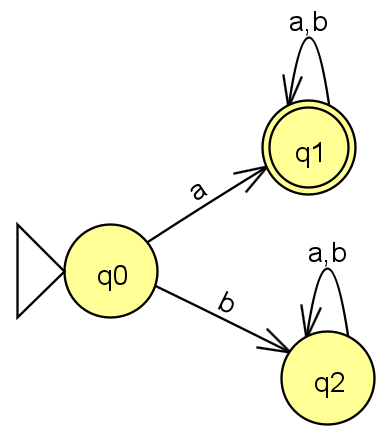
\includegraphics[width=0.2\textwidth]{../../../images/DFAs/ex1_q1.png}



% \vspace{3cm}
% \begin{flushleft}
% أرجو لكم وقتًا ممتعًا.

% الأستاذ محمود اغبارية.
% \end{flushleft}


% \end{document}


\title{أساسيات البرمجة كائنية التوجه في \textenglish{C\#}}

\begin{document}

\maketitle
\thispagestyle{fancy}

%=============================================================
\section{الفصل الأول: بناء الفئات والتعامل مع الكائنات}
%=============================================================

\begin{itemize}[itemsep=5pt]
    \item \textbf{الفئة} (\textenglish{Class}): قالب أو مخطط مجرد يحدد شكل ونوع الكائن. يشمل تعريف الفئة، الترويسة، واتفاقيات التسمية (\textenglish{Naming Conventions}).
    \item \textbf{الخصائص} (\textenglish{Attributes}): متغيرات تُعرّف داخل الفئة لوصف حالة الكائن، وتشمل التوصيف، التعريف، والتهيئة.
    \item \textbf{الأساليب} (\textenglish{Methods}): دوال تحدد سلوك الكائن، وتشمل التوقيع (\textenglish{Signature})، تمرير البارامترات، والقيم المرجعة.
    \item \textbf{إنشاء الكائنات} (\textenglish{Instantiation}): استخدام الكلمة المحجوزة \textenglish{new} لحجز مساحة وإنشاء نسخة في الذاكرة.
    \item \textbf{دالة البناء} (\textenglish{Constructor}): دالة خاصة لتهيئة الكائن عند إنشائه، وتشمل دالة البناء الافتراضية (\textenglish{Default Constructor}) ودالة البناء الناسخة (\textenglish{Copy Constructor}).
    \item \textbf{المتغيرات المرجعية} (\textenglish{References}): متغيرات تؤشر إلى عنوان الكائن في الذاكرة ولا تحتويه مباشرة. يشمل ذلك تمرير الكائنات كبارامترات.
    \item \textbf{تواصل الكائنات} (\textenglish{Object Communication}): استخدام الكائنات القائمة والتواصل بينها عبر صيغة النقطة (\textenglish{Dot Notation}).
    \item \textbf{الكائنات المركبة} (\textenglish{Complex Objects}): كائنات تحتوي بداخلها على كائنات أخرى كخصائص.
    \item \textbf{التحميل الزائد} (\textenglish{Method Overloading}): كتابة نفس الدالة ببارامترات مختلفة داخل نفس الفئة.
    \item \textbf{استخدام المكتبات الجاهزة} (\textenglish{API}): التعامل مع مكتبات الفئات القياسية واستخدامها في البرنامج.
\end{itemize}

%=============================================================
\section{الفصل الثاني: المفاهيم الهيكلية المتقدمة وتغليف البيانات}
%=============================================================

\begin{itemize}[itemsep=5pt]
    \item \textbf{المصفوفات ككائنات} (\textenglish{Arrays as Objects}): التعامل مع المصفوفة (أحادية وثنائية الأبعاد) ككائن برمجي له خصائص وأساليب، ومعالجة استثناءات تجاوز حدود المصفوفة (\textenglish{Out of Bounds})، وإنشاء مصفوفات من الكائنات.
    \item \textbf{فئة النصوص} (\textenglish{String Class}): التعامل مع السلاسل النصية ككائنات، واستخدام أساليبها المختلفة، ومعامل الدمج (\textenglish{Concatenation})، واستخدام دالة \textenglish{ToString()} لتمثيل الكائن نصياً.
    \item \textbf{استدعاء الفئات} (\textenglish{Using/Import}): جلب واستخدام فئات من مساحات أسماء أخرى لتوسيع قدرات البرنامج.
    \item \textbf{الأعضاء الساكنة} (\textenglish{Static Members}): خصائص وأساليب تابعة للفئة كقالب عام وليس للنسخ (الكائنات)، ويشمل ذلك فئات الخدمة (\textenglish{Utility Classes}).
    \item \textbf{محددات الوصول} (\textenglish{Access Modifiers}): تحديد صلاحيات القراءة والتعديل باستخدام \textenglish{public} و \textenglish{private}.
    \item \textbf{التغليف وإخفاء المعلومات} (\textenglish{Encapsulation}): حماية البيانات الداخلية للفئة، والفصل الواضح بين واجهة الاستخدام (\textenglish{Interface}) وتفاصيل التنفيذ الداخلي (\textenglish{Implementation}).
    \item \textbf{توثيق الكود} (\textenglish{Documentation}): استخدام التعليقات المخصصة (مثل \textenglish{XML Docs} أو \textenglish{Javadoc}) لتوثيق الدوال والفئات لتسهيل استخدام الواجهات البرمجية.
\end{itemize}

\end{document}